% this file is called up by thesis.tex
% content in this file will be fed into the main document

%: ----------------------- introduction file header -----------------------
\chapter{Identification and Analysis Techniques}
\label{chap:methods}

% the code below specifies where the figures are stored
\ifpdf
    \graphicspath{{5/figures/PNG/}{5/figures/PDF/}{5/figures/}}
\else
    \graphicspath{{5/figures/EPS/}{5/figures/}}
\fi


% ----------------------------------------------------------------------
%: ----------------------- introduction content ----------------------- 
% ----------------------------------------------------------------------
% Quote here (if required)



\noindent 
\\ {\it 
You see, but you do not observe. The distinction is clear.
\begin{flushright}
Sir Arthur Conan Doyle (A Scandal in Bohemia) \\
\end{flushright}
 }


\vspace{15mm}
Coronal bright fronts are typically observed as broad diffuse features in coronal emission lines as previously discussed in Chapter~\ref{chap:cbfs}. This diffuse nature makes it difficult to identify CBF pulses in individual images, complicating analysis of the phenomenon. These issues have resulted in the development of several different image processing techniques for identifying CBFs, each with advantages and disadvantages. It is shown here that the techniques traditionally used for identifying CBFs are fundamentally flawed and prone to undefined user--dependent errors. A new semi--automated technique is proposed for the rigorous identification of CBF pulses.

Once the pulse has been identified in subsequent images a thorough analysis requires a determination of the pulse kinematics. These can be derived using several different methods, either by direct numerical differentiation of the data or alternatively through the application of a model fit to the data. Again, each technique has drawbacks, particularly when dealing with the typical data-set sizes that are encountered when studying CBFs. 

In this chapter, the issues traditionally associated with identifying CBF pulses are discussed. The different image processing techniques used are presented in Section~\ref{subsect:diff_imgs} with a semi--automated technique for identifying CBFs outlined in Section~\ref{subsect:cor_pita}. The different numerical techniques that can be used to derive the pulse kinematics directly from distance--time measurements are then presented in Section~\ref{subsect:num_diff} with an examination of the effects of image cadence and pulse uncertainty outlined in Section~\ref{subsect:img_cad}. It is shown that the errors associated with the identification and analysis of CBFs can be minimised through the use of a percentage base difference image processing technique allied to a model fit using a bootstrapping approach.


\section{Pulse Identification}
\label{sect:identify_pulse}

The diffuse nature of CBFs has made them difficult to observe in single images, with identification improved in movies as a consequence of their motion. To overcome this issue, CBFs have traditionally been identified using difference images, an approach which involves subtracting one image from another in a bid to highlight the moving pulse. There are several different types of difference images including the running difference (RD), base difference (BD) and percentage base difference (PBD) techniques.


\subsection{Difference Imaging}
\label{subsect:diff_imgs}

Difference imaging is a simple image processing technique that is designed to highlight relative motion in images, making it particularly useful for identifying CBF pulses in subsequent images. Some examples of a differencing approach can be seen in Figures~\ref{fig:may1997} and \ref{fig:rd_images}, both of which show a CBF pulse highlighted using differencing.

\begin{figure}[!t]
\begin{center}
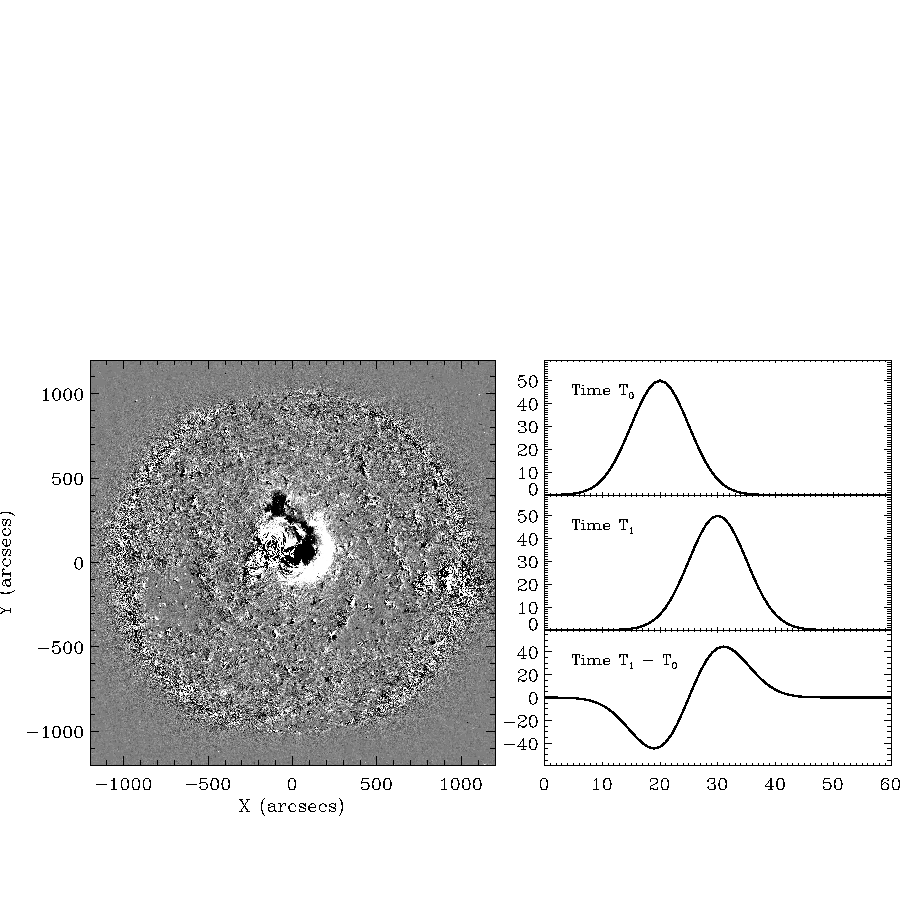
\includegraphics[clip=,trim=0mm 10mm 0mm 60mm,width = 0.95\textwidth]{rd_images}
\caption{\emph{Left}: Running difference image from 2007~May~19. White (black) is a positive (negative) intensity change relative to the previous image. \emph{Right}: Simulated intensity profiles showing a pulse at T$_{0}$ (top panel) T$_{1}$ (middle panel) and T$_{1}$ - T$_{0}$ (bottom panel).}
\label{fig:rd_images}
\end{center}
\end{figure}

The most common and simplest technique used to accentuate the pulse signature is the running difference image. This involves subtracting a following image from a leading image (i.e.,\ $\Delta I = I_{t} - I_{t-1}$), highlighting relative motion with an increase in intensity seen in white and a decrease in intensity seen in black (as shown in the left-hand panel of Figure~\ref{fig:rd_images} and in Figure~\ref{fig:diff_imgs}). While this technique does a good job of highlighting the moving pulse, there are a number of issues that must be kept in mind when examining the resulting images \citep[see also][for some additional issues with the misinterpretation of RD images]{Attrill:2010ab}.

As shown in the right-hand panel of Figure~\ref{fig:rd_images}, the profile of the pulse seen in a RD image does not necessarily conform to that of the original pulse. The technique highlights the relative intensity change between images, which allows the general rather than specific motion of the pulse to be discerned. The nature of the data being analysed means that the resulting RD image will also have to be scaled to make the pulse apparent. This scaling is entirely user dependent and strongly influences the apparent size of the observed pulse. 

\begin{figure}[!t]
\begin{center}
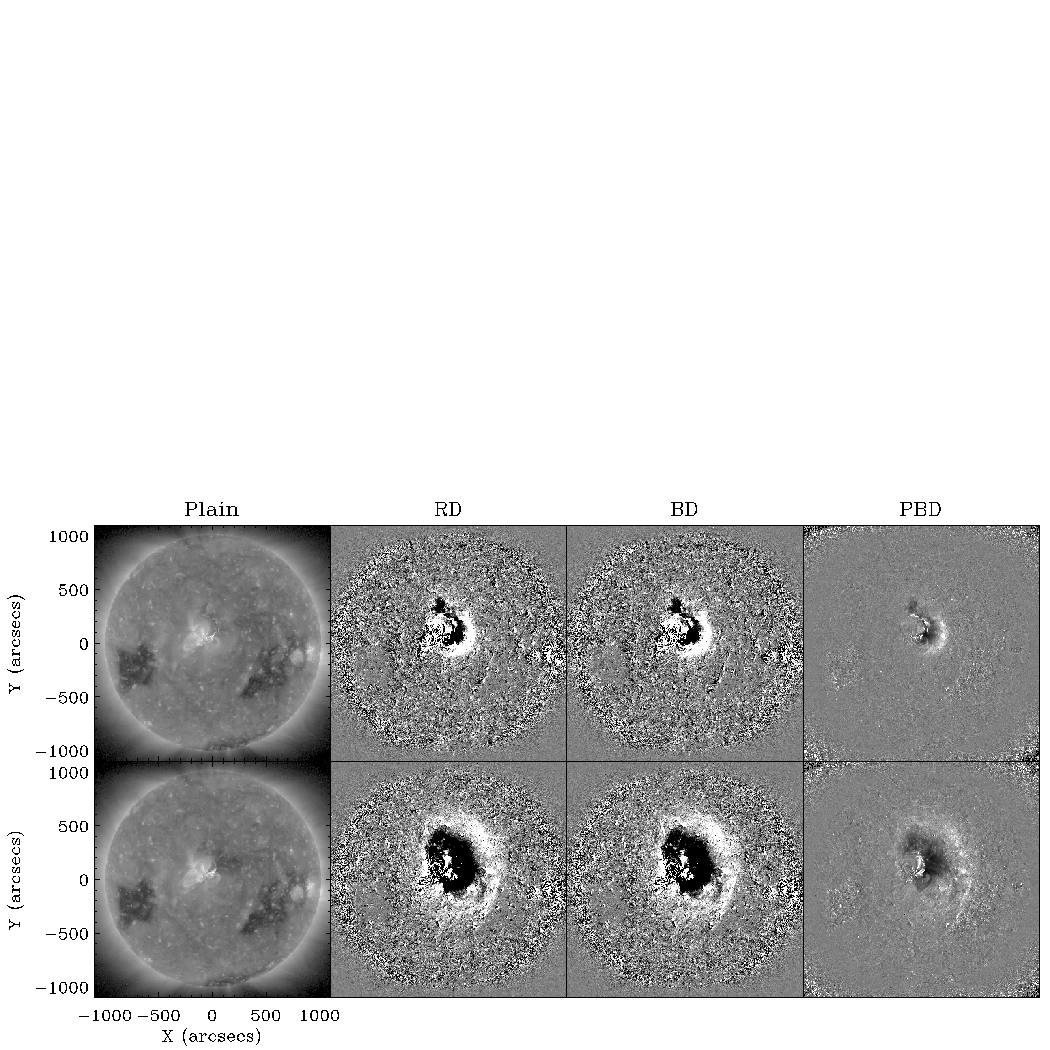
\includegraphics[clip=,trim=0mm 0mm 0mm 84mm,width = 0.99\textwidth]{diff_imgs}
\caption{Plain, running difference (RD), base difference (BD) and percentage base difference (PBD) images for the times 12:52:00~UT (top row) and 13:02:00~UT (bottom row) on 2007~May~19 in the 195~\AA\ passband from \emph{STEREO}-A. The plain image is shown using logarithmic scaling, the RD and BD images using user-defined intensity scaling and the PBD image using its inherent intensity  scaling (i.e., $-$100\% to 100\%).}
\label{fig:diff_imgs}
\end{center}
\end{figure}

An alternative technique proposed to negate the influence of image--to--image variation is the base difference (BD) technique (see Figure~\ref{fig:diff_imgs}). Here, a pre-event image is subtracted from each subsequent image, highlighting the intensity changes relative to the pre-event image (i.e.,\ $\Delta I = I_{t} - I_{0}$). This is designed to remove only the coronal background, allowing an easier identification of the pulse itself. Although this does a better job of enhancing the pulse signature, the small-scale background structure of the corona is also highlighted using this technique. Consequently, this technique becomes ineffective over long timescales with the resulting image difficult to interpret.

The BD technique is also subject to user-defined scaling which can over-emphasise the pulse signature, while the diffuse nature of the pulse compared to the small-scale motion also highlighted by the technique means that image smoothing is often required. While this makes the pulse easier to identify, it does introduce an additional error that must be accounted for when identifying the pulse position.

A variation on this technique was originally proposed by \citet{Wills-Davey:1999ve} and involves dividing the BD image by the pre-event image (i.e.,\ $\Delta I = (I_{t} - I_{0})/I_{0} \times 100$ (see Figure~\ref{fig:diff_imgs}). This produces images with a relative intensity ranging from $-100$\% to 100\%, eliminating the possibility of arbitrary image scaling. The peak pulse intensity is also then given as a percentage of the pre-event intensity, allowing a better comparison from frame to frame. While this variation eliminates the issues with regard to the arbitrary image scaling, the assumption about a quiet pre-event coronal background remain.

One additional approach to minimising the errors associated with the individual differencing technique is to account for the effects of the differential rotation of the Sun. This can be done by de-rotating all images to the same pre-event time before applying the differencing techniques. While the timescale of a CBF pulse is quite short, the de-rotation allows the errors associated with the small-scale coronal features to be minimised. This has the effect of reducing the additional error at the pulse edges due to small--scale coronal movements and solar rotation, allowing a better identification of the pulse.

\subsection{Automated Pulse Identification Techniques}
\label{subsect:cor_pita}

Once identification of the pulse has been confirmed in a difference image, the next step in the pulse analysis is to determine the distance of the pulse from a defined source point at a given time. The traditional approach for this has been to use a point--and--click identification of the edge of the pulse using a RD or BD image with a user--defined scaling. However, as shown in Figure~\ref{fig:pulse_scaling}, the scaling used for the image defines the position and width of the pulse.

\begin{figure}[!t]
\begin{center}
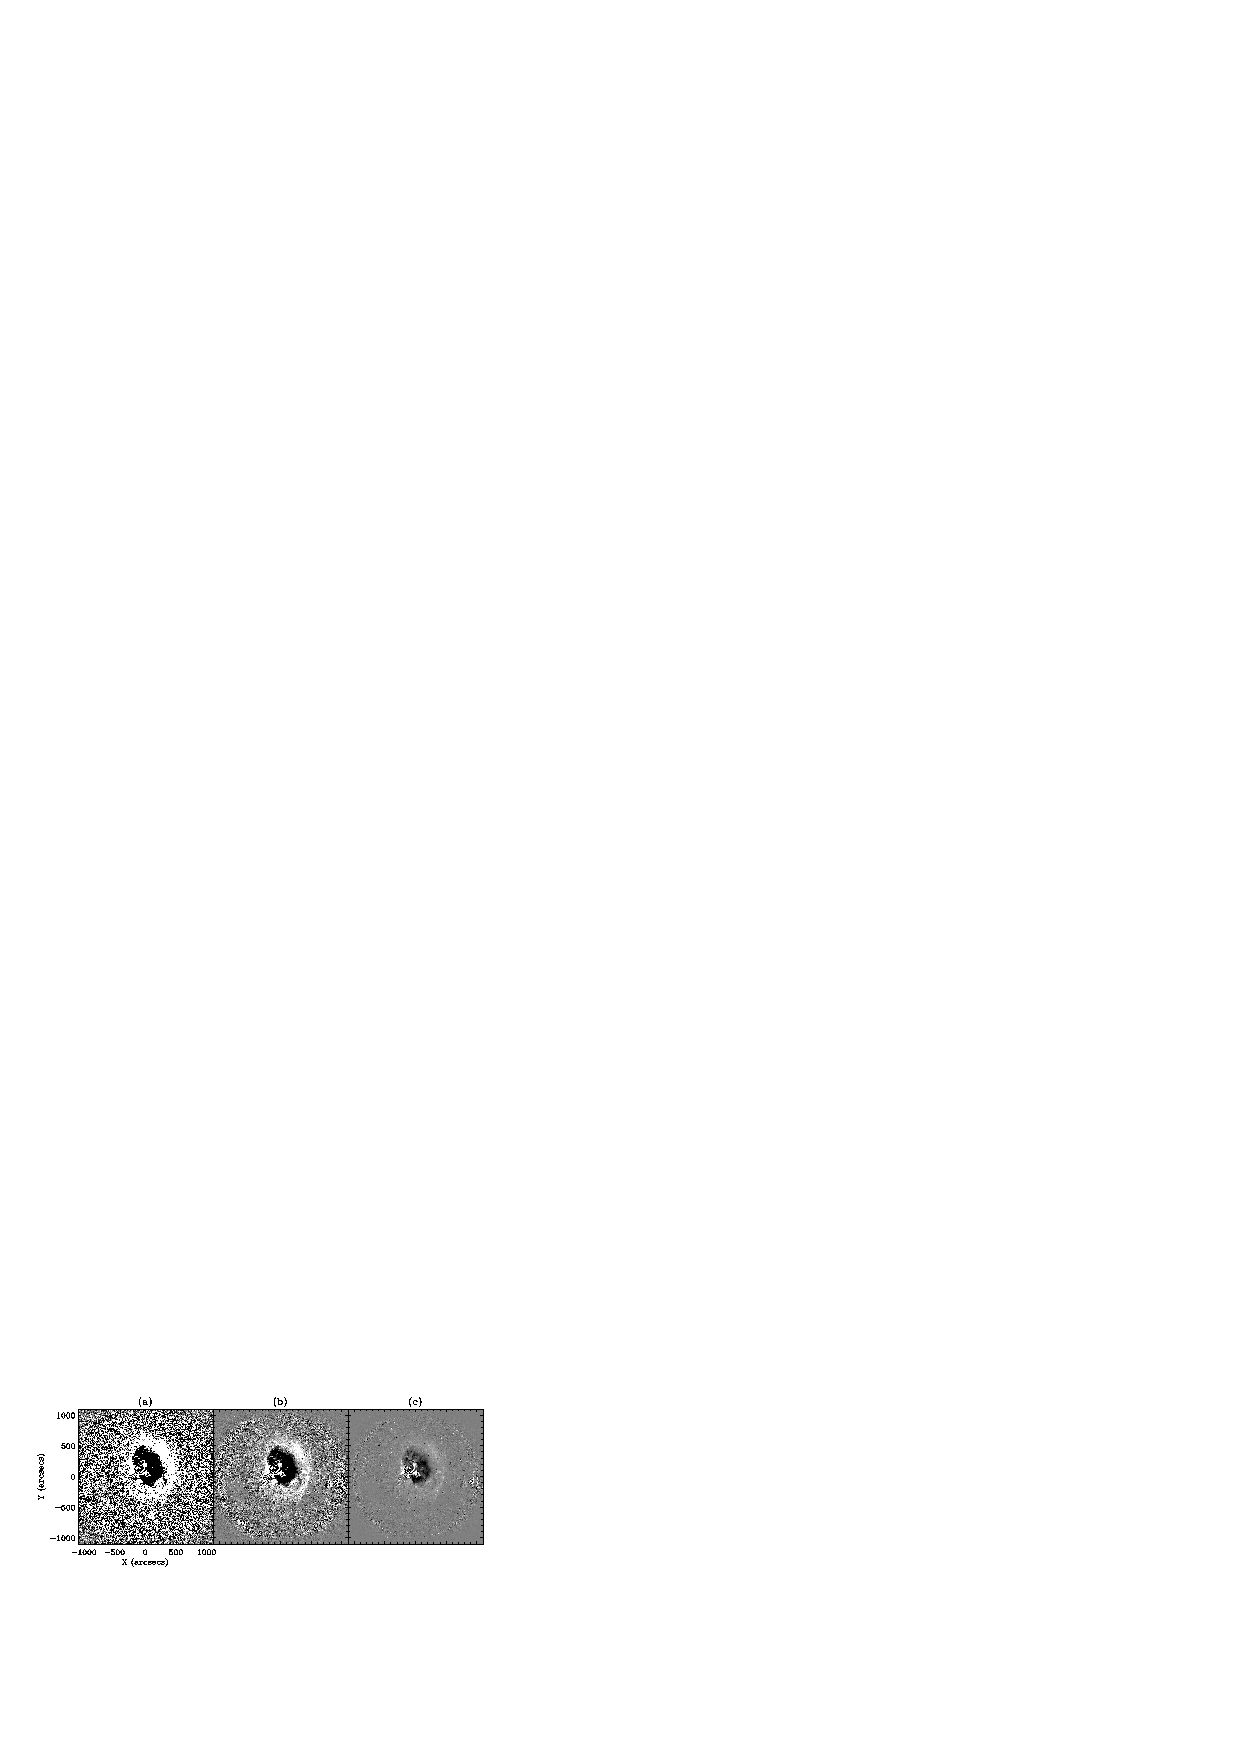
\includegraphics[clip=,trim=0mm 0mm 0mm 47mm,width = 0.99\textwidth]{pulse_scaling}
\caption{Running difference images with variable photon flux intensity scaling of (a) $\pm$1, (b) $\pm$10 and (c) $\pm$50.}
\label{fig:pulse_scaling}
\end{center}
\end{figure}

It is apparent from Figure~\ref{fig:pulse_scaling} that the pulse is most apparent when a harsh (i.e., $\pm1$) scaling is applied to the image. However, while this highlights the full extent of the pulse, it also results in an increase in the small--scale variation of the background corona. An additional problem with point--and--click pulse identification is defining the location on the pulse to be identified. This is generally the front edge of the pulse. However, it is clear from Figure~\ref{fig:pulse_scaling} that this varies with the scaling chosen. Consequently, point--and--click pulse identification is highly user--dependent, and not an efficient technique for a detailed analysis of CBFs. 

A more effective approach is to take an intensity profile across the pulse and identify the location of the peak intensity of the pulse, effectively allowing the centre of the pulse to be tracked rather than the edge. Whereas the edge of the pulse is loosely defined and highly variable, CBFs have been noted as having a roughly Gaussian shape \citep{Wills-Davey:1999ve}, meaning that the pulse centre is a more statistically significant indicator of the pulse position.

A technique was devised to allow semi--autonomous identification of the CBF pulse using derotated percentage base difference images. This approach was chosen as the inherent scaling of the technique used to produce them mitigated against any user--defined assumptions, while the derotation allowed the small--scale coronal variation to be minimised. To ensure that the signal--to--noise of the pulse was maximised, a great-circle sector (i.e., an area on the sphere bounded by two great circles) projected onto the Sun was defined with the source point of the pulse defined as the crossing point of the great circles. The intensity within this sector could then be averaged across the arc (in annuli of increasing radii with 1~degree width on the surface of the sphere) to produce an intensity profile as a function of distance away from the source location \citep[cf. similar techniques proposed by][]{Warmuth:2004ab,Podladchikova:2005ab,Wills-Davey:2006ab,Veronig:2010ab}.

To minimise the errors associated with identification of the source point, the first two observations of the CBF pulse in the 171 and 195~\AA\ passbands were fitted using an ellipse, with the mean centres of the four ellipses taken as the source point of the CBF pulse. The orientation of the arc sector was then chosen to maximise the number of pulse identifications for a given event, with an arc of 30~degrees chosen as this provided the greatest signal while minimising errors resulting from any change in the propagation direction of the pulse.

\begin{figure}[!t]
\centering{
              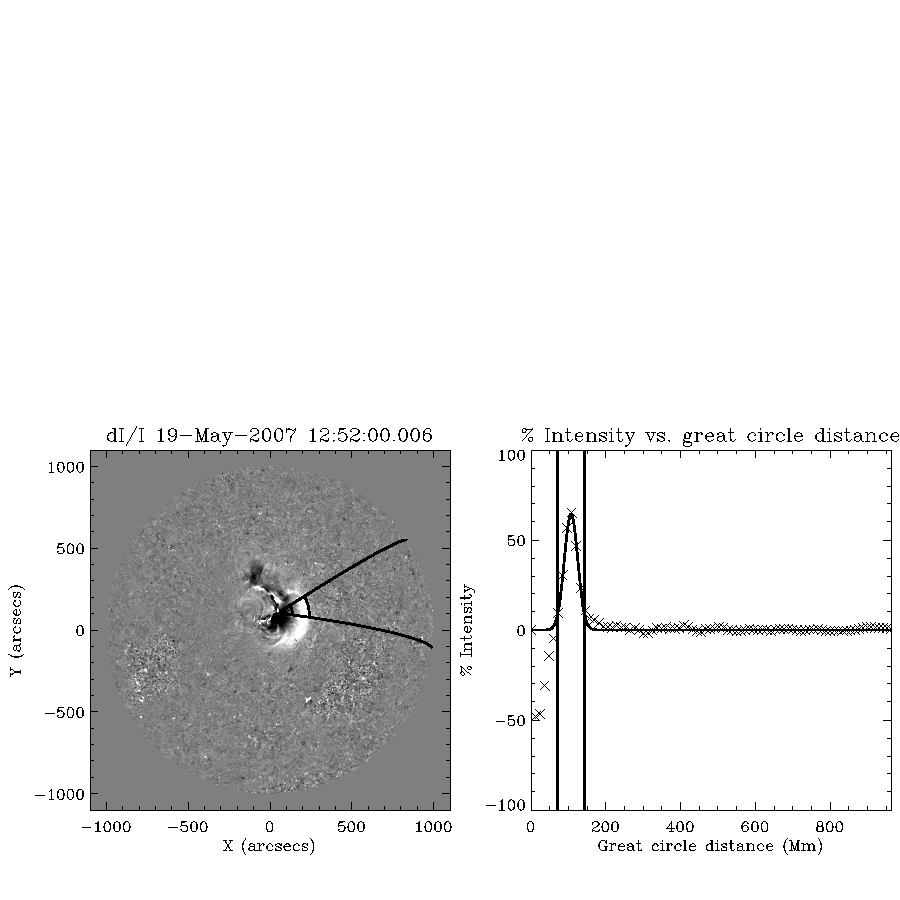
\includegraphics[width=0.99\textwidth,clip=,trim=0mm 5mm 0mm 70mm]{pbd_img_profile}
              }
\caption{\emph{Left panel}: PBD image with arc sector over-plotted. \emph{Right panel}: Intensity profile across arc sector. The intensity profile at a given distance corresponds to the mean intensity across the arc sector at that distance. This is then fitted using a Gaussian model and repeated for the next image. The vertical lines in the right-hand plot and arc lines in the left-hand plot correspond to the $2\sigma$ limits of the Gaussian fit.}
\label{fig:algorithm}
\end{figure}

Figure~\ref{fig:algorithm} shows how the algorithm works for the event from 2007~May~19 as observed by \emph{STEREO}-A. The left--hand panel shows the PBD image with the arc sector overplotted, while the right--hand panel shows the 1--dimensional intensity profile along the arc sector. The pulse is clearly visible in the arc sector, and has been fitted using a Gaussian model allowing the $2\sigma$ limits of the fit to be overplotted as arc--lines in the left--hand panel and vertical lines in the right--hand panel.

This process is repeated for each observation of the pulse, allowing the variation with time of the distance of the pulse from the source to be examined. This can then be used to determine the kinematics of the pulse, while the temporal variation in the pulse width can be studied for evidence of pulse broadening. The next step is to identify the optimal technique for deriving the pulse kinematics for a small data--set such as that typically produced by \emph{STEREO}/EUVI observations of a CBF.

\section{Statistical Analysis}
\label{sect:stats}

As well as minimising the errors associated with the actual identification of the CBF pulse, it was important to identify the optimum method for deriving the kinematics of the pulse. To do this, a number of different numerical differencing techniques and a residual resampling bootstrapping approach were tested and compared. This was required as a result of the sparse nature of the data obtained from \emph{STEREO}/EUVI in addition to concerns with regard to the approach previously used to derive the pulse kinematics.

\begin{figure}[!hp]
\begin{center}
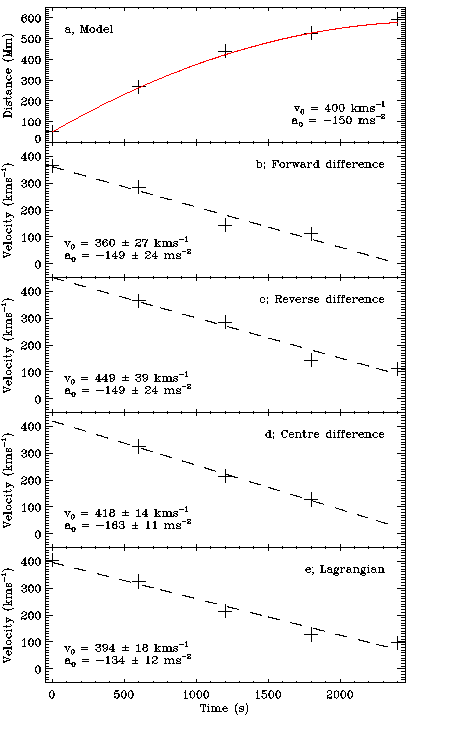
\includegraphics[clip=,trim=0mm 5mm 5mm 0mm,width = 0.78\textwidth]{num_diff}
\caption{\emph{Panel} (\emph{a}); Simulated data set (asterisks) with the model kinematics shown by the red line and given in the bottom right. \emph{Panels} (\emph{b})--(\emph{e}); Velocity derived using forward--difference (b), reverse--difference (c), centre--difference (d) and Lagrangian difference (e) techniques. The kinematics determined by the fitted dashed line are shown in the bottom left in each case.}
\label{fig:num_diff}
\end{center}
\end{figure}

\subsection{Numerical Differencing}
\label{subsect:num_diff}

The simplest way to determine the pulse kinematics given distance--time measurements is to use a numerical differencing technique to directly derive the velocity and acceleration of the pulse. Here, four different numerical differencing techniques were identified; a forward, reverse and centre difference method, all of which can be derived using a Taylor expansion, and a three-point Lagrangian interpolation technique. To allow a direct comparison between the different techniques, a simulated data--set was created (shown in panel a of Figure~\ref{fig:num_diff}), with the numerical differencing techniques used to estimate the known kinematics.

This simulated data--set was constructed using an equation of the form,
\begin{equation}
r(t) = r_0 + v_0 t + \frac{1}{2}a t^2 + \delta r
\end{equation}
with $r_0 = 50$~Mm, $v_0 = 400$~kms$^{-1}$ and $a = -150$~ms$^{-2}$. The $\delta r$ term here corresponds to $\sim$5\% noise which was added to the simulated data to reproduce observational variations. An observing cadence of 600~s was also used as this is the typical observing cadence of \emph{STEREO}. The resulting simulated data--set is shown as the asterisks in panel (a) of Figure~\ref{fig:num_diff}, with the known kinematics shown as the red line. This simulated data set was then used to compare the different numerical differencing techniques.


\subsubsection{Forward Differencing}
\label{subsubsect:f_diff}

The first numerical differencing technique to be tested was the forward-difference technique. This involves the computation of the derivative at the point $r[t + \Delta t]$ by extrapolating forward from the point $r[t]$. The derivative can be determined using the Taylor series,
\begin{equation}
r[t + \Delta t] = r[t] + r[t]'\Delta t +  \frac{r[t]''}{2!}(\Delta t)^{2} + \frac{r[t]'''}{3!}(\Delta t)^{3}  + ... \label{eqn:f_diff_0}
\end{equation}
By rearranging this equation, it is possible to find the derivative at time t, 
\begin{equation}
r[t]' = \frac{r[t + \Delta t] - r[t]}{\Delta t} -  \frac{r[t]''}{2!}(\Delta t) - \frac{r[t]'''}{3!}(\Delta t)^{2}  + ... \label{eqn:f_diff_1}
\end{equation}
Although this series continues to infinity, the correction values are dominated by the term of order $\Delta t$. As a result, this is usually written as,
\begin{equation}
r[t]' = v[t] = \frac{r[t + \Delta t] - r[t]}{\Delta t} + O(\Delta t) \label{eqn:f_diff_2}
\end{equation}
where $O(\Delta t)$ is the truncation error term. This can also be used to derive the acceleration in a similar fashion by replacing $r$ with $v$ to give,
\begin{equation}
v[t]' = \frac{v[t + \Delta t] - v[t]}{\Delta t} + O(\Delta t). \label{eqn:f_diff_3}
\end{equation}
However, $v[t]$ is already known from Equation~\ref{eqn:f_diff_2} above, so by substituting this into Equation~\ref{eqn:f_diff_3}, it is possible to derive the acceleration $a[t]$ as,
\begin{equation}
a[t] = \frac{r[t + 2\Delta t] - 2r[t+\Delta t] + r[t]}{\Delta t} + O(\Delta t)^2 . \label{eqn:f_diff_4}
\end{equation}
Equations~\ref{eqn:f_diff_2} and \ref{eqn:f_diff_4} can then be used to determine the instantaneous velocity and acceleration at the point $r[t]$ for each value of $t$. 

This approach does have some issues which make it unsuitable for analysing CBF observations. The technique calculates the derivative assuming a straight line gradient between points, while the final data point is negated with each iteration as an inherent consequence of the method. This approach is also particularly susceptible to point--to--point variations, with the result that noisy data can produce strongly varying velocity and acceleration estimates.

The results of the forward--difference technique are shown in panel (b) of Figure~\ref{fig:num_diff}. The effects of the point--to--point variation are very apparent, while the inherent nature of the technique has removed the final data point. The kinematics obtained by fitting the data points also show a strong underestimation of $v_0$, while there are large errors associated with the estimates of both $v_0$ and $a$.

\subsubsection{Reverse Differencing}
\label{subsubsect:r_diff}

The reverse differencing approach uses a similar methodology, although in this case the derivative at the point $r[t-\Delta t]$ is calculated by extrapolating backwards from the point $r[t]$. This can be determined using the Taylor series expansion,
\begin{equation}
r[t - \Delta t] = r[t] - r[t]'\Delta t +  \frac{r[t]''}{2!}(\Delta t)^{2} - \frac{r[t]'''}{3!}(\Delta t)^{3}  + ... \label{eqn:r_diff_0}
\end{equation}
Once again, this equation can be rearranged to find the derivative at time $t$,
\begin{equation}
r[t]' = \frac{r[t] - r[t - \Delta t]}{\Delta t} +  \frac{r[t]''}{2!}(\Delta t) - \frac{r[t]'''}{3!}(\Delta t)^{2}  + ... \label{eqn:r_diff_1}
\end{equation}
The correction values here are again dominated by the term of order $\Delta t$, allowing this equation to be rewritten as,
\begin{equation}
r[t]' = v[t] = \frac{r[t] - r[t - \Delta t]}{\Delta t} + O(\Delta t) \label{eqn:r_diff_2}
\end{equation}
where $O(\Delta t)$ is the truncation error term. As before, the acceleration term can also be derived by replacing $r$ with $v$ to give,
\begin{equation}
v[t]' = \frac{v[t] - v[t - \Delta t]}{\Delta t} + O(\Delta t). \label{eqn:r_diff_3}
\end{equation}
Again, $v[t]$ is already known from Equation~\ref{eqn:r_diff_2} above, so by substituting this into Equation~\ref{eqn:r_diff_3}, the acceleration $a[t]$ can be derived in terms of $r[t]$ as,
\begin{equation}
a[t] = \frac{r[t] - 2r[t-\Delta t] + r[t - 2\Delta t]}{\Delta t} + O(\Delta t)^2 . \label{eqn:r_diff_4}
\end{equation}
Both equation~\ref{eqn:r_diff_2} and \ref{eqn:r_diff_4} can then be used to determine the instantaneous velocity and acceleration at the point $r[t]$ for each value of $t$. 

Panel (b) in Figure~\ref{fig:num_diff} shows the result of this analysis for the simulated data--set. The reverse--difference approach is very similar to the forward--difference technique, and this is reflected in the derived data--points which have identical velocity values albeit at a different time. Once again, the point--to--point variation is significant, while the first data--point has also been removed. The fitted kinematics show a higher estimated initial velocity but identical acceleration, with the initial velocity not corresponding to that of the original model.

The same caveats that apply to the forward difference technique also apply to the reverse difference technique due to their inherent similarities in using two adjacent points ($r[t]$ \& $r[t+\Delta t]$ and $r[t]$ \& $r[t-\Delta t]$ for the forward and reverse difference respectively) to determine the derivative at a given point. Both techniques are quite simplistic and as a result are only applicable in simplistic cases. Both techniques also remove points from either edge with each iteration as an inherent consequence of the technique. As a result, neither technique is appropriate for determining the kinematics of a CBF pulse.

\subsubsection{Centre Differencing}
\label{subsubsect:c_diff}

A more accurate approach that utilises the Taylor series methodology is the centre difference technique. This uses the points either side of the point under examination $r[t]$ (i.e.,\ $r[t - \Delta t]$ and $r[t + \Delta t]$), smoothing the data and producing a more accurate estimate of the numerical derivative at that point. The Taylor series at the points $r[t - \Delta t]$ and $r[t + \Delta t]$ respectively are defined as,
\begin{align}
r[t - \Delta t] = r[t] - r[t]'\Delta t +  \frac{r[t]''}{2!}(\Delta t)^{2} - \frac{r[t]'''}{3!}(\Delta t)^{3}  + ... \label{eqn:c_diff_0_0} \\
r[t + \Delta t] = r[t] + r[t]'\Delta t +  \frac{r[t]''}{2!}(\Delta t)^{2} + \frac{r[t]'''}{3!}(\Delta t)^{3}  + ... \label{eqn:c_diff_0_1}
\end{align}
as shown previously in Equations~\ref{eqn:f_diff_0} and \ref{eqn:r_diff_0} above. The centre difference approach subtracts Equation~\ref{eqn:c_diff_0_0} from Equation~\ref{eqn:c_diff_0_1} to produce,
\begin{equation}
r[t + \Delta t] - r[t - \Delta t] = 2 r[t]'\Delta t +  2 \frac{r[t]'''}{3!}(\Delta t)^{3}  + ... ,
\end{equation}
which can then be rearranged in terms of $r[t]'$ to give,
\begin{equation}
r[t]' = \frac{r[t + \Delta t]- r[t - \Delta t]}{2\Delta t} +  \frac{r[t]'''}{3!}(\Delta t)^{2}  + ... 
\end{equation}
Following the notation from before, this can be rewritten as,
\begin{equation}
r[t]' = v[t] = \frac{r[t + \Delta t] - r[t - \Delta t]}{2\Delta t} + O(\Delta t^{2})
\end{equation}
where $O(\Delta t^{2})$ is the truncation error term. The instantaneous acceleration term $a[t]$ can then be determined as,
\begin{equation}
r[t]'' = a[t] = \frac{r[t + \Delta t] - 2r[t] + r[t - \Delta t]}{(\Delta t)^2} + O(\Delta t^{2})
\end{equation}
This allows the instantaneous velocity and acceleration at the point $r[t]$ to be determined. 

The results of applying this technique to the simulated data--set are shown in Panel (d) of Figure~\ref{fig:num_diff}. The centre--difference technique produces a smoother estimation of the kinematics than the forward-- and reverse--difference and the fitted kinematics are closer to the model values. However, the centre difference technique does remove both of the edge points as an inherent consequence of its operation. 

Despite producing a better estimate of the pulse kinematics, the inherent issues of the centre--difference technique are a cause for concern. The removal of edge points makes analysis of the kinematics difficult, particularly when considering that a given \emph{STEREO}/EUVI observation of a CBF event may have only 3 or 4 distance--time estimates. Consequently, the centre difference technique is usually unsuitable for this analysis.


\subsubsection{Lagrangian Differencing}
\label{subsubsect:l_diff}

A more advanced technique for determining the derivative at a point numerically is the three-point Lagrangian interpolation technique used by the built-in \emph{deriv.pro} routine in IDL. This method uses three adjacent points ($r[t-\Delta t]$, $r[t]$ and $r[t+ \Delta t]$) to fit a Lagrangian polynomial function of the form,
\begin{align}
P(x) &= \frac{(x - t)(x - (t+\Delta t))}{((t-\Delta t) - t)((t-\Delta t) - (t+\Delta t))}r[t-\Delta t] \nonumber \\
&+ \frac{(x - (t-\Delta t))(x - (t+\Delta t))}{(t - (t-\Delta t))(t - (t+\Delta t))}r[t] \nonumber \\ 
&+ \frac{(x - (t-\Delta t))(x - t)}{((t+\Delta t) - (t-\Delta t))((t+\Delta t) - t))}r[t+\Delta t]
\end{align}
where $x$ is the abscissa of the point $r[t]$. The derivative of this is then given by,
\begin{align}
P'(x) &= \frac{2x - t - (t+\Delta t)}{((t-\Delta t) - t)((t-\Delta t) - (t+\Delta t))}r[t-\Delta t] \nonumber \\
&+ \frac{2x - (t-\Delta t) - (t+\Delta t))}{(t - (t-\Delta t))(t - (t+\Delta t))}r[t] \nonumber \\ 
&+ \frac{2x - (t-\Delta t) - t)}{((t+\Delta t) - (t-\Delta t))((t+\Delta t) - t))}r[t+\Delta t]
\end{align}
By substituting $t$ for $x$, the polynomial used to determine the derivative $P'(t)$ is given as,
\begin{equation}
P'(t) = \frac{1}{2\Delta t}(r[t+\Delta t] - r[t-\Delta t])
\end{equation}

This approach does not assume a straight line gradient between points (unlike the forward, reverse and centre difference techniques above), while also compensating for edge points by increasing the errors and retaining all of the original data points. The Lagrangian technique also smoothes the data, removing the spiky appearance produced by the Taylor series expansion techniques. This is apparent in panel (e) of Figure~\ref{fig:num_diff}, where the Lagrangian technique has retained all data--points.

Despite this, there are a number of issues associated with this approach, in particular as a result of the small data sets associated with these disturbances. The cadence of \emph{STEREO}/EUVI means that there are typically only 4 or 5 observations of a CBF pulse per event, of which three are required to determine the numerical derivative of one data point. The combination of this with the interpolation at the edges has the effect of skewing the edge points, giving the impression of kinematic variation that may not be real. This can be seen in the fit to the derived Lagrangian kinematics in panel (e) of Figure~\ref{fig:num_diff}, where the edges points have strongly influenced an underestimation of the kinematics. 

This skewing effect strongly suggests that the Lagrangian interpolation technique is inappropriate for the small data-sets typically obtained for CBF analysis. The problems associated with each numerical differencing approach studied here indicates that an alternative method must be used to determine the kinematics of a CBF pulse. A possible alternative is the fitting of a specified model to the distance-time measurements, although once again the small data-sets available can make this difficult. 

\subsection{Effects of Image Cadence and Positional Uncertainty}
\label{subsect:img_cad}

In the absence of a numerical technique to determine the kinematics of a CBF pulse, the cadence of the observing instrument and the degree of uncertainty in the data must also be considered. Here, the influence of both cadence and uncertainty are examined using the simulated data discussed in Section~\ref{subsect:num_diff}. The effects of varying image cadence were the first to be examined; this is shown in Figures~\ref{fig:num_diff_cad} and \ref{fig:num_diff_vary_cad}. 

\begin{figure}[!t]
\begin{center}
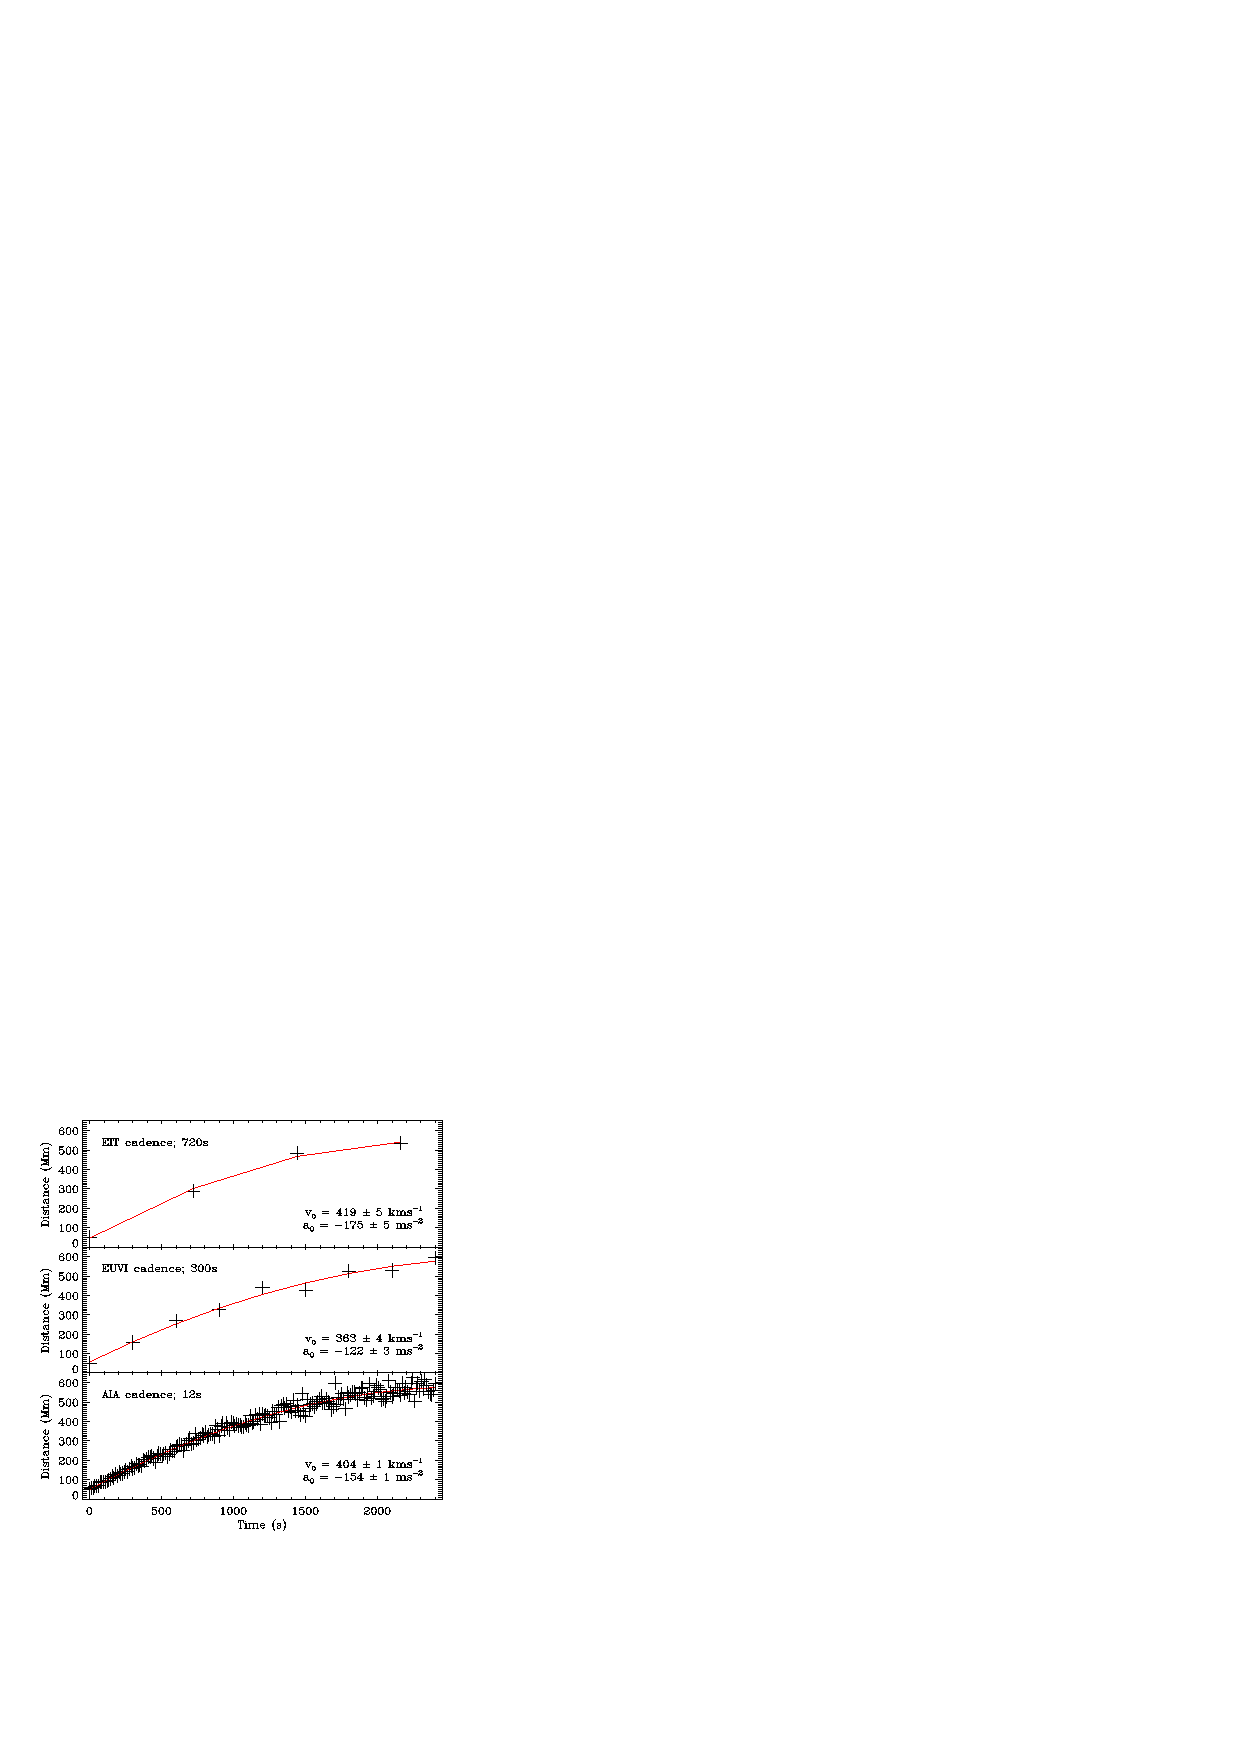
\includegraphics[clip=,trim=0mm 5mm 0mm 0mm,width = 0.95\textwidth]{num_diff_cad}
\caption{Simulated data (crosses) for cadences of 720~s (\emph{top}; comparable to EIT), 300~s  (\emph{middle}; comparable to EUVI) and 12~s  (\emph{bottom}; comparable to AIA). In each case, the fit to the data is shown in red with derived kinematics in the bottom right of each panel.}
\label{fig:num_diff_cad}
\end{center}
\end{figure}

The same data--set was used for each of the panels shown in Figure~\ref{fig:num_diff_cad}, with the cadence varied to best reflect data from \emph{SOHO}/EIT (top panel at 720~s), \emph{STEREO}/EUVI (middle panel at 300~s) and \emph{SDO}/AIA (bottom panel at 12~s). The derived kinematics are given in the bottom right of each panel with the fit to the data shown by the red line. It is immediately apparent that the higher cadence data allows a better fit to the data despite the uncertainty in the data (which was kept at $\pm$5\% of the model for each data--set). This implies that higher cadence data is required to derive the true kinematics of a CBF pulse.

\begin{figure}[!t]
\begin{center}
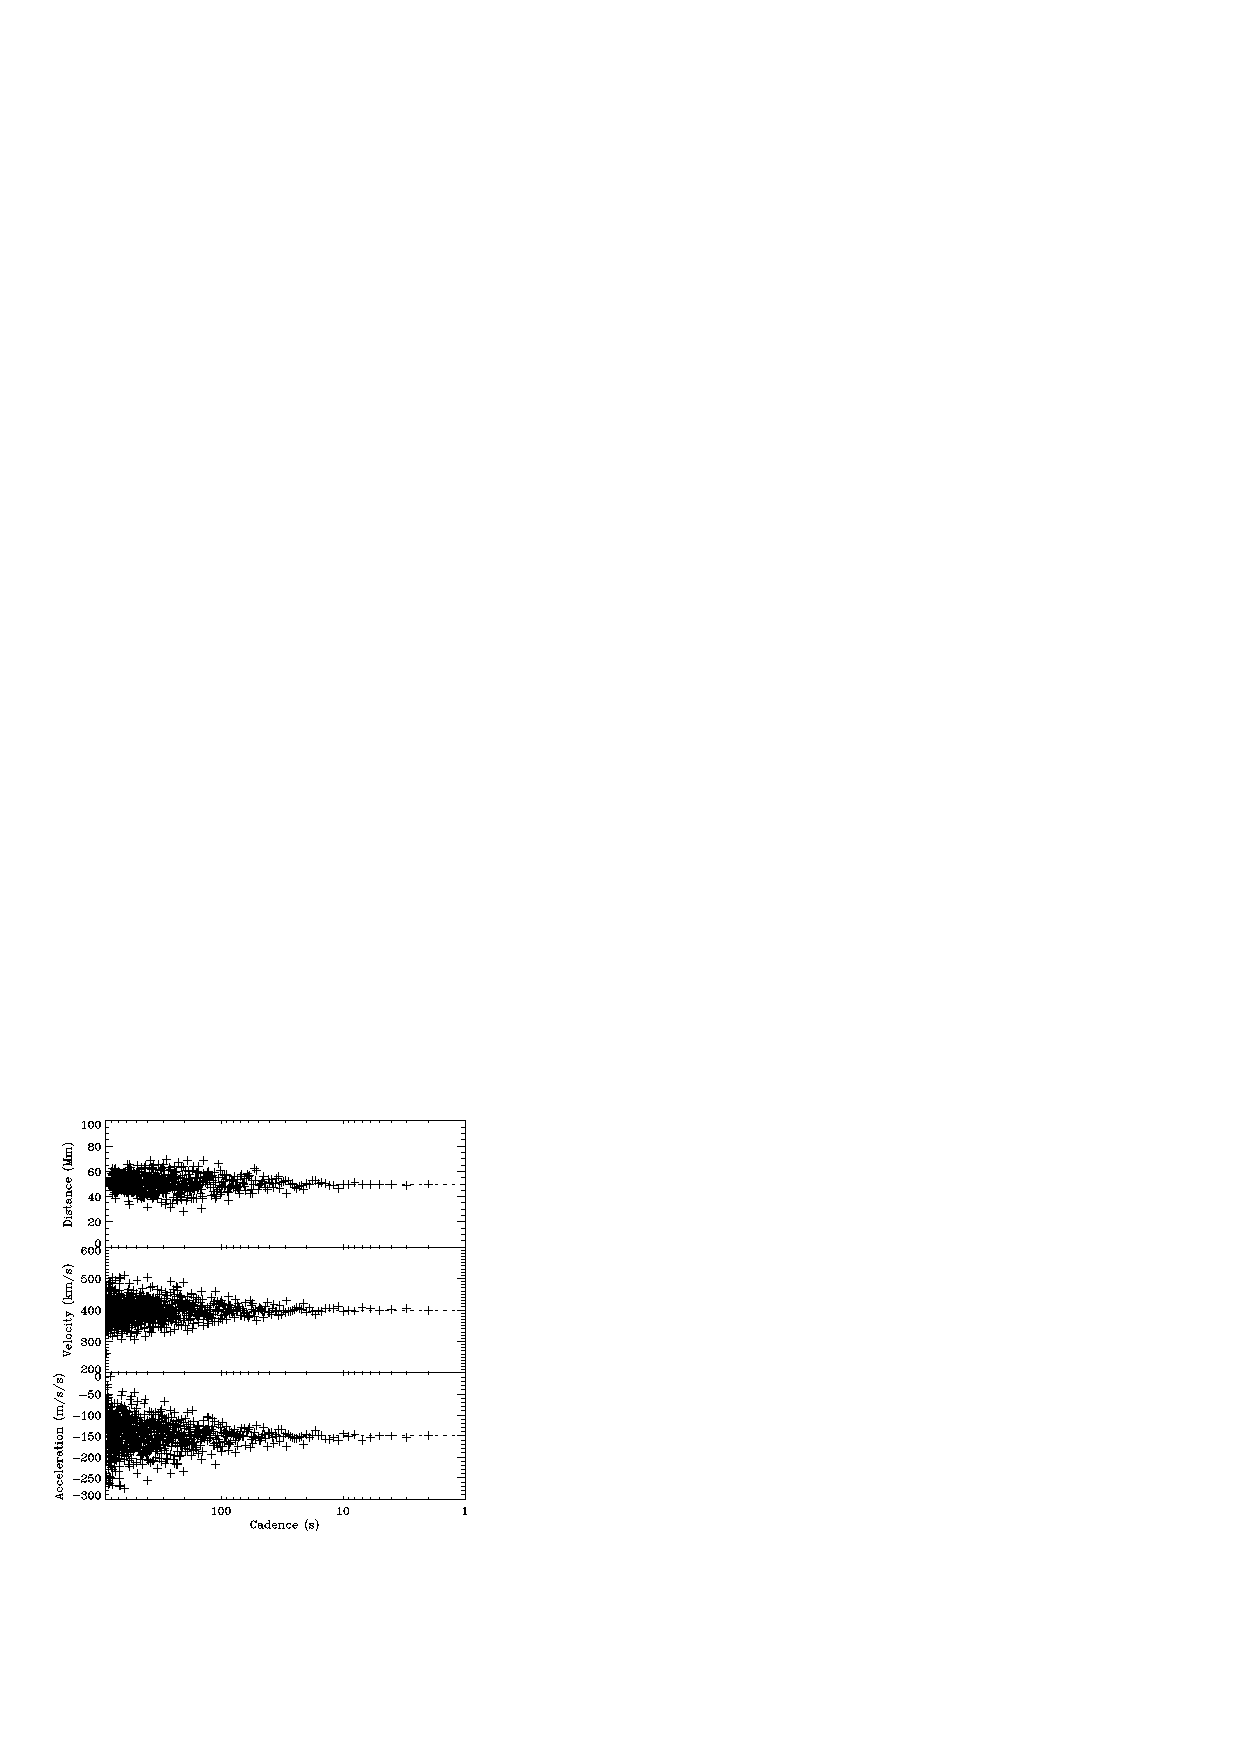
\includegraphics[clip=,trim=0mm 5mm 0mm 0mm,width = 0.95\textwidth]{num_diff_vary_cad}
\caption{Derived kinematics for varying image cadence with $\pm$5\% uncertainty. Distance, velocity and acceleration are shown in the top, middle and bottom panels respectively, with the x--axis shown using logarithmic scaling to highlight the effects of varying the image cadence.}
\label{fig:num_diff_vary_cad}
\end{center}
\end{figure}

The variation in derived kinematics with cadence is shown in Figure~\ref{fig:num_diff_vary_cad} (again for $\pm$5\% uncertainty). As the cadence decreases, the derived velocity and acceleration approach the model values, with the scatter showing a dramatic reduction below $\sim$50~s cadence. These results are consistent with the observations made by both \citet{Long:2008eu} and \citet{Ma:2009ab} and show that the effects of image cadence must be accounted for when trying to derive the true kinematics of a CBF pulse.

\begin{figure}[!t]
\begin{center}
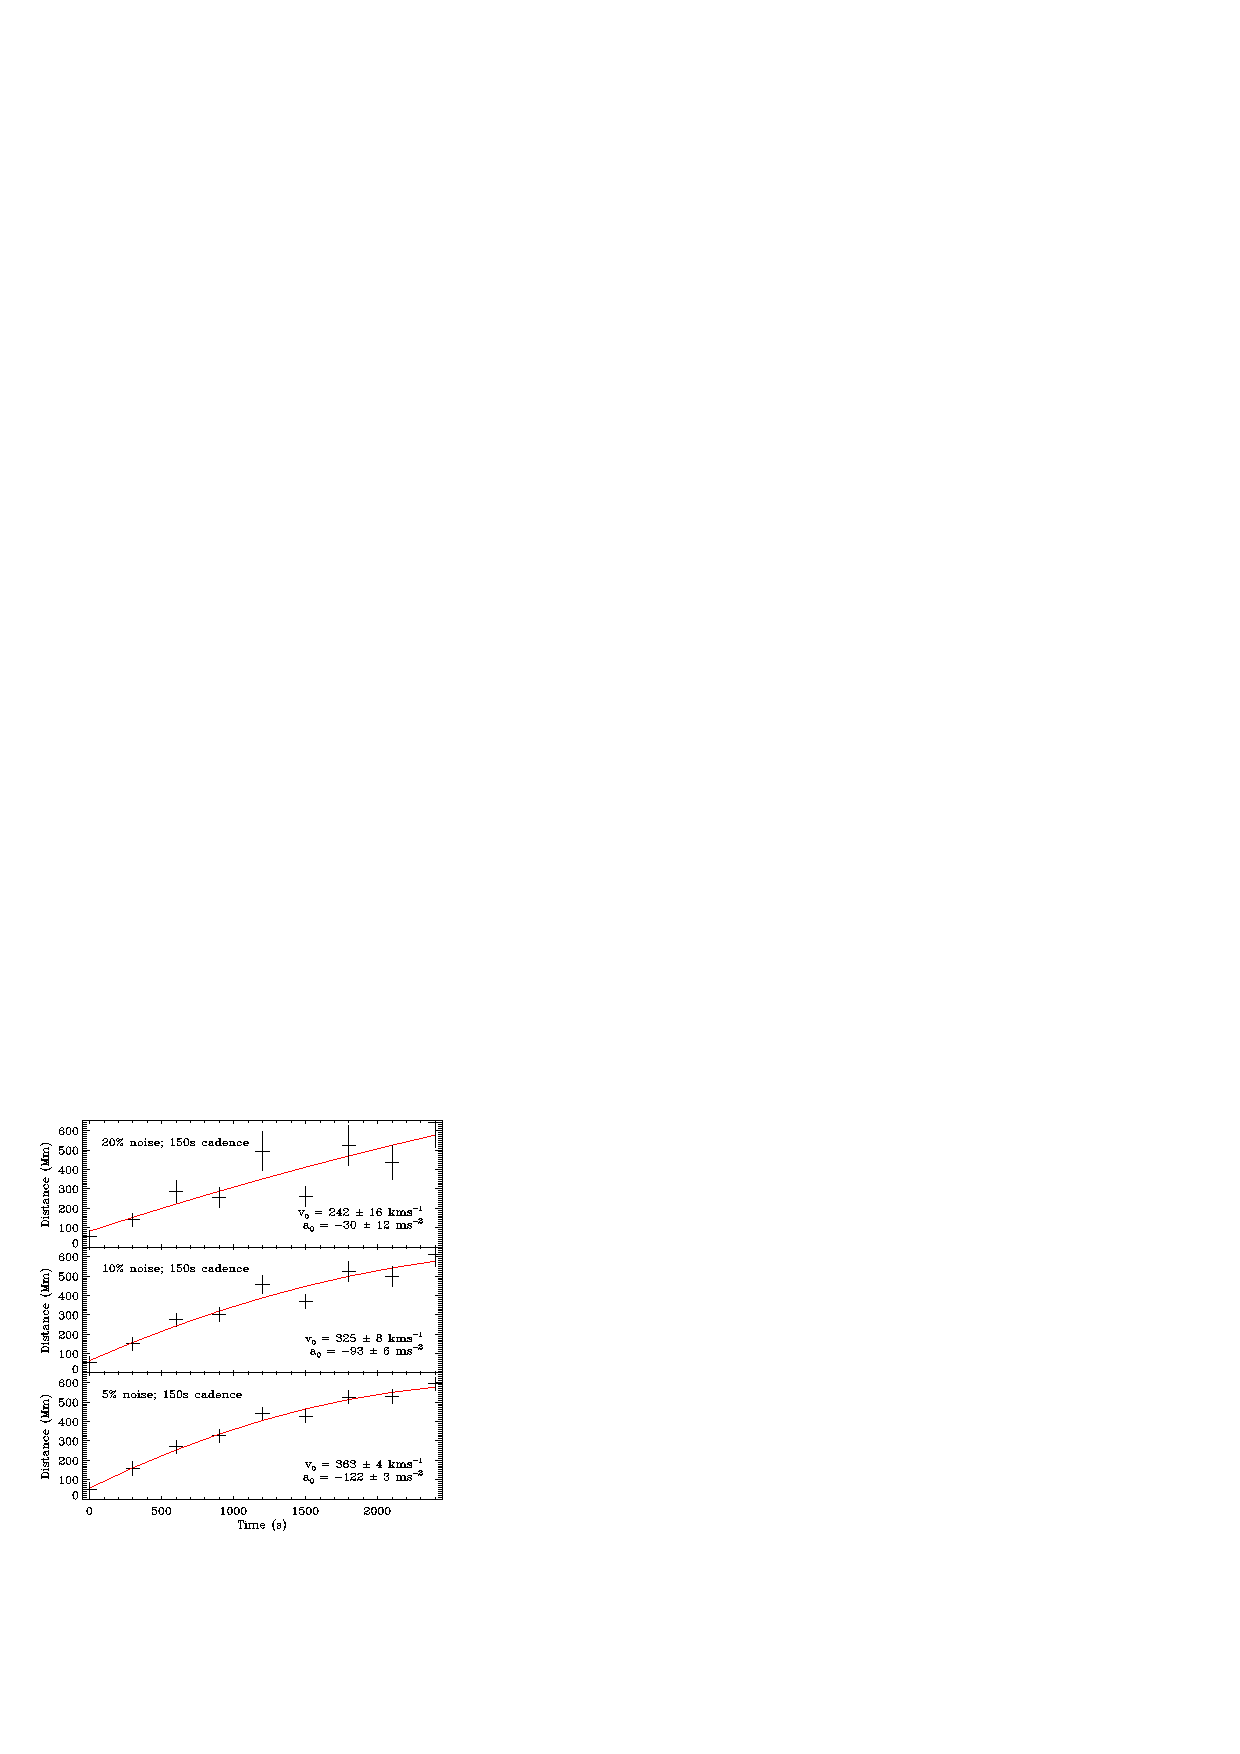
\includegraphics[clip=,trim=0mm 5mm 0mm 0mm,width = 0.95\textwidth]{num_diff_noise}
\caption{Simulated data (crosses) for noise distributions with widths of $\pm$20\% (\emph{top}), $\pm$10\%  (\emph{middle}) and $\pm$5\%  (\emph{bottom}) of the data value. In each case, the fit to the data is shown in red with derived kinematics in the bottom right of each panel.}
\label{fig:num_diff_noise}
\end{center}
\end{figure}

The effects of varying uncertainty in the data were also examined for constant image cadence with the results of this analysis shown in Figures~\ref{fig:num_diff_noise} and \ref{fig:num_diff_vary_noise}. Figure~\ref{fig:num_diff_noise} shows the derived kinematics for the simulated data--set with the top panel showing uncertainties of $\pm$20\%, the middle panel showing uncertainties of $\pm$10\% and the bottom panel showing uncertainties of $\pm$5\%. The variation in uncertainty has a noticeable effect on the derived kinematics in each case, with the acceleration in particular exhibiting significant variation with uncertainty. 

\begin{figure}[!t]
\begin{center}
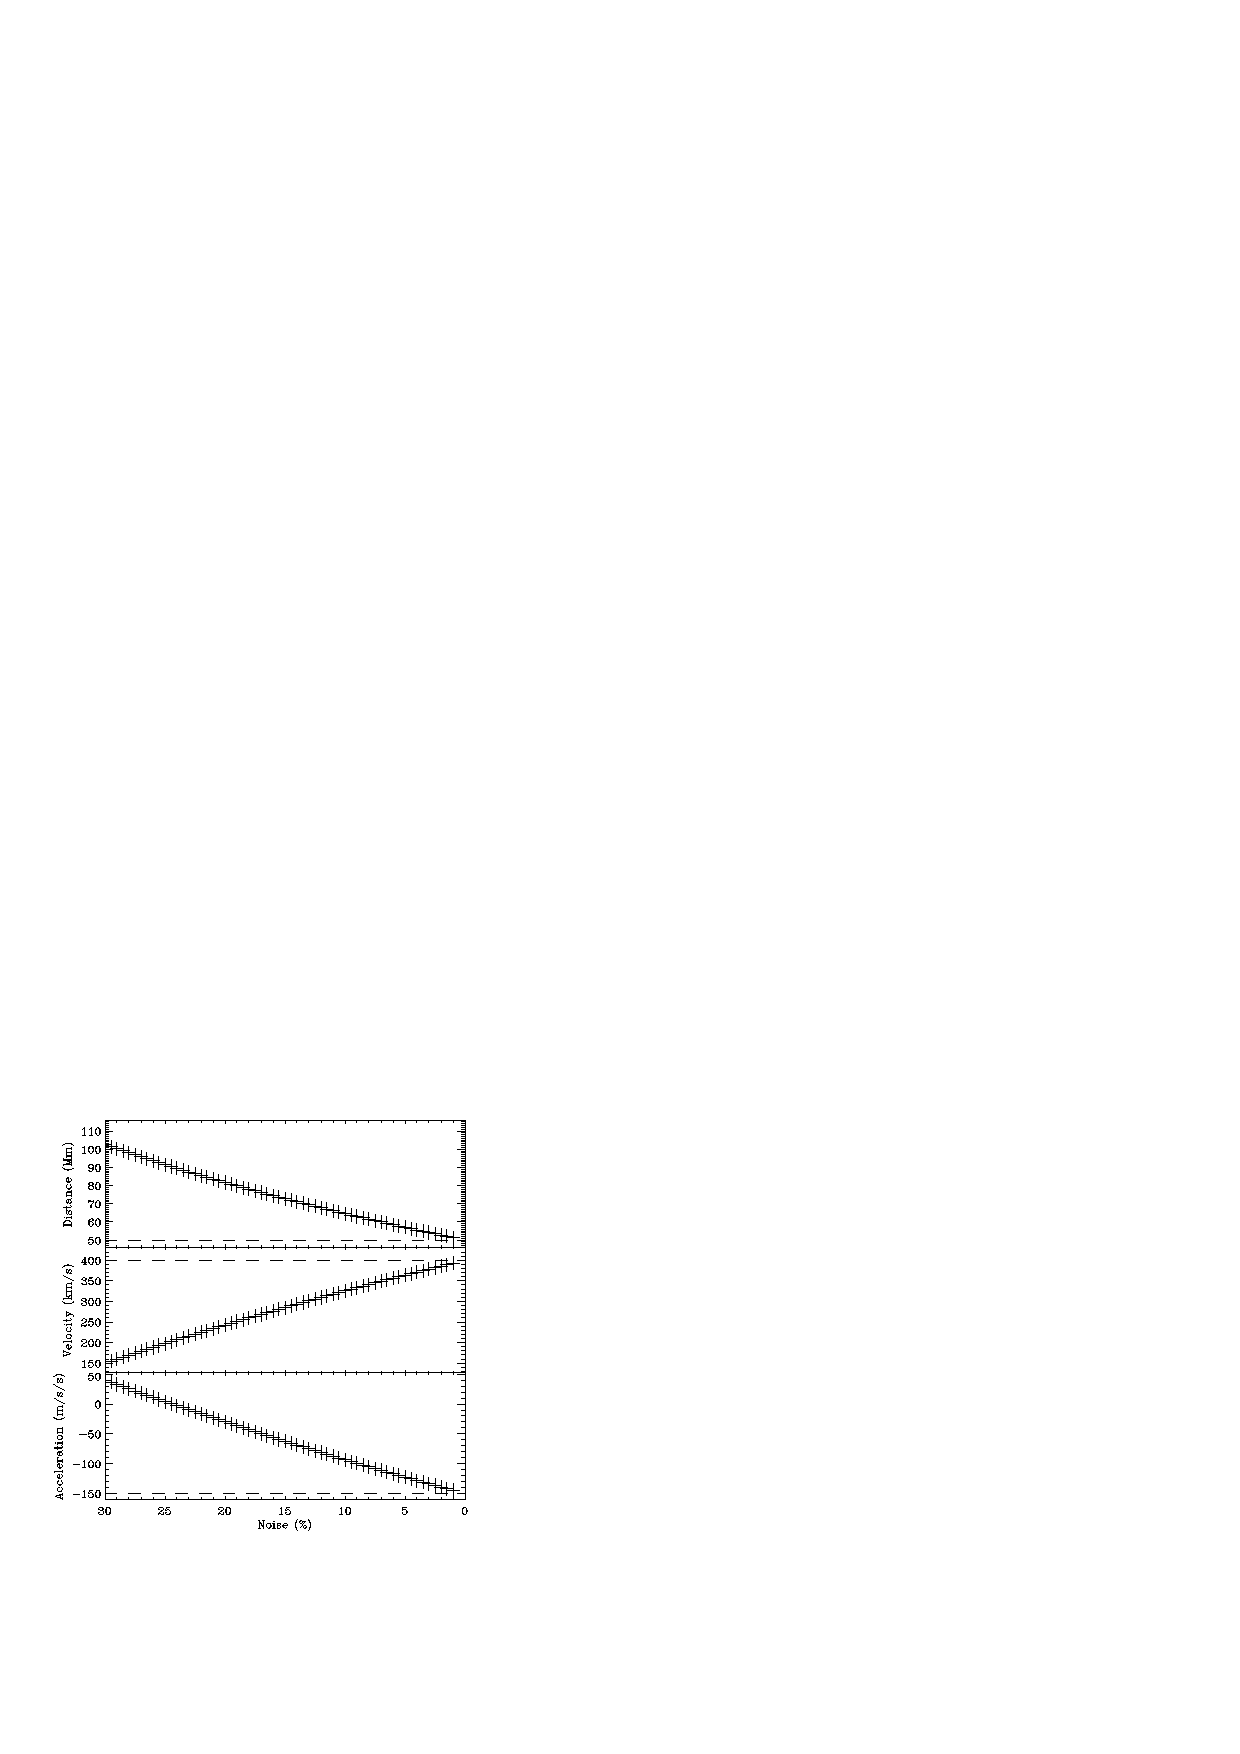
\includegraphics[clip=,trim=0mm 5mm 0mm 0mm,width = 0.95\textwidth]{num_diff_vary_noise}
\caption{Derived kinematics for varying uncertainty at 150~s image cadence. Distance, velocity and acceleration are shown in the top, middle and bottom panels respectively.}
\label{fig:num_diff_vary_noise}
\end{center}
\end{figure}

The variation in the derived kinematics with uncertainty is shown in Figure~\ref{fig:num_diff_vary_noise}, with the variation in offset distance (r$_{0}$), initial velocity (v$_{0}$) and acceleration (a$_{0}$) shown in the top, middle and bottom panels respectively. Some variation is apparent in each case, with the acceleration again showing the strongest variation. The derived kinematics are seen to approach the model kinematics as the noise reduces to 0\% as expected. 

It is clear that the variation in both noise and imaging cadence can strongly influence the derived kinematics of a CBF pulse, while the different numerical differencing techniques do not return accurate estimates of the pulse kinematics. However, it is possible to use a bootstrapping approach to overcome these issues as this is a statistically significant technique that has been optimised for small data-sets such as those typically obtained when studying CBF pulses. 


\subsection{Bootstrapping}
\label{subsect:bootstrap}

\begin{figure}[!t]
\begin{center}
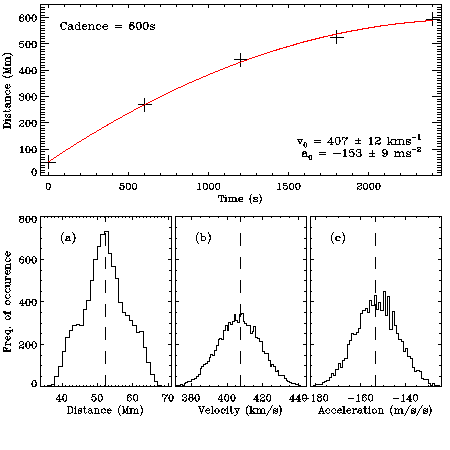
\includegraphics[clip=,trim=0mm 5mm 0mm 0mm,width = 0.95\textwidth]{bootstrap}
\caption{\emph{Top}: Simulated data (asterisks) with bootstrapped fit shown in red and parameters in bottom right. \emph{Bottom}: Histograms showing the distance (a), velocity (b) and acceleration (c) derived using the bootstrapping technique.}
\label{fig:bootstrap}
\end{center}
\end{figure}

Bootstrapping was first proposed by \citet{Efron:1979p1831} as a general interpretation of the jackknife, allowing statistical quantities to be estimated from a limited sample to a high degree of accuracy. In principle this allows a statistical quantity (such as the mean, variance etc.) of a distribution to be estimated using a small sample of measurements from that distribution. The resulting estimates are statistically significant, with statistically defined associated error estimates. 

While there are a number of different bootstrapping techniques, each of which is useful for a different purpose, in this case we will be using the residual resampling technique. Whereas the majority of bootstrapping techniques involve removing one point at random and recalculating the fit to the data, this is inappropriate in this case due to the small sample set available. The residual resampling technique however, does not require data-point removal, making it more appropriate for small data-sets such as those available here.

The residual resampling technique works as follows. The distance-time measurements ($y_i$; $i=1, 2, \ldots, n$) are first fitted using a quadratic equation of the form
\begin{equation}
r(t) = r_0 + v_0 t + \frac{1}{2}a t^2,
\end{equation}
where $r_0$ is the offset distance, $v_0$ is the initial velocity, $a$ is the constant acceleration of the pulse, and $t$ is the time elapsed since the first observation of the disturbance. This yields the fitted values ($\hat{y_{i}}$) and residuals ($\hat{\epsilon}=y_{i} - \hat{y_{i}}$) for each point. The residuals are then randomly ordered and randomly assigned a sign ($1$ or $-1$), before being added to the original fit values to produce a new data set. These new data are then fitted using the same model, with the resulting re-fitted parameters recorded. The process is then repeated a large number of times ($\sim$10\,000).

This has the effect of repeating the fit to slightly varying data a large number of times, allowing a distribution of fit values to be obtained. The mean and standard deviation of this distribution then provide the estimated value and associated error of the parameter. This technique is statistically rigorous and produces a more accurate result than a simple model fit to the given data. 

This technique was applied to the simulated data--set used in Section~\ref{subsect:num_diff} to allow a comparison of the effectiveness of the bootstrapping approach with the numerical differencing techniques. The results of this analysis are shown in Figure~\ref{fig:bootstrap}. The upper panel here shows the simulated data (indicated by the asterisks) with the bootstrapped fit to the data shown by the red line. The kinematics obtained by the bootstrapping approach are given in the bottom right. The bottom panels (a), (b) and (c) show the histograms for the distance, velocity and acceleration parameters respectively. These histograms returned by the bootstrapping approach for each parameter allow a statistical determination of the fit parameters, a fact reflected in the error term for the derived kinematics. 

The kinematics returned by the bootstrapping approach match the model kinematics within one standard deviation, while also producing an accurate estimate with well--defined errors, unlike those of the numerical differencing techniques. It should also be noted that none of the data--points have been removed, unlike the majority of the numerical differencing techniques tested. 

As a result of the simulations carried out to test the different approaches to determining the kinematics of a CBF pulse, the residual resampling bootstrapping technique was chosen as the best method. This fits a model directly to the distance--time measurements, allowing the kinematics of the CBF pulse to be determined to a high degree of accuracy. The kinematics given for each future event studied here therefore reflects the mean value of the bootstrapped distribution, with the associated error given by the standard deviation.

\section{Conclusions}
\label{sect:methods_conc}

As outlined in this chapter, there are many different issues beyond the simple identification and analysis of the pulse that must be examined and accounted for when studying CBFs. The choice of technique used to identify the pulse can have a strong effect on the estimated pulse parameters, while the resulting kinematics are influenced by the technique used to estimate them. The cadence of the observations and the uncertainty in the pulse position (which is influenced by the resolution of the instrument) can also affect the derived kinematics.

Of the different image processing technique considered here, the percentage base difference images offer the optimum approach for identifying the CBF pulse. This technique removes the background corona, highlighting the actual pulse rather than an intensity change relative to the previous observation. The inherent scaling afforded by the percentage intensity approach also removes any ambiguity with regard to the identification of the pulse. 

The combination of PBD images with the semi--automated algorithm presented here allows the CBF pulse to be identified in an unbiased way, negating the user--defined errors associated with traditional methods of pulse identification. The algorithm also uses a consistent approach to identify the pulse, with the use of a Gaussian model ensuring that the pulse position and width are comparable from both image to image and event to event. This will allow a direct comparison of multiple events and represents a opportunity to systematically examine CBFs.

Once the CBF pulse has been identified and tracked, the next step involves determining the pulse kinematics. This has traditionally been done using numerical differencing techniques, but it has been shown here that this approach is incompatible with the typical cadence of CBF observations. The different numerical differencing techniques based on a Taylor expansion approach remove data points as a direct consequence of their operation, while the Lagrangian interpolation approach is strongly affected by the edge points. 

The derived kinematics have also been shown to be strongly affected by the cadence of the observations and the associated uncertainty of the pulse position. By comparing derived kinematics for a simulated data--set using cadences comparable to those available from \emph{SOHO}/EIT, \emph{STEREO}/EUVI and \emph{SDO}/AIA it was shown that the derived kinematics approached those of the model as the cadence decreased. This indicates that it will be possible to derive the true kinematics of a CBF pulse using high cadence data from \emph{SDO}/AIA. The uncertainty in pulse position also influences the derived kinematics, with a decrease in the positional uncertainty producing derived kinematics that approach those of the model.

The issues surrounding the pulse identification and derivation of the resulting kinematics can be negated by combining the semi--automated algorithm presented here with a residual--resampling bootstrapping technique. This allows any errors associated with the identification of the CBF pulse to be minimised while also producing statistically significant estimates of the pulse kinematics with defined associated errors.  This approach is used to examine a series of CBF events observed using the \emph{STEREO} spacecraft in the next chapter.